\begin{frame}{Raisonneur}{Généralités}
	\begin{itemize}
		\item Prise de décision
		\item Valuation des formes connues
		\item Découverte de nouvelles formes
	\end{itemize}
\end{frame}

\begin{frame}{Raisonneur}{Moteur de choix}
	\begin{minipage}{0.45\textwidth}
		\only<1|handout:0>{
			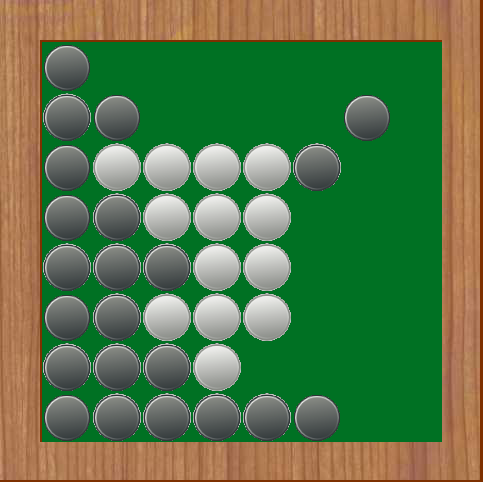
\includegraphics[width=0.8\textwidth]{img/screenshoot/raisonneur_choix_0}	
		}
		\only<2|handout:0>{
			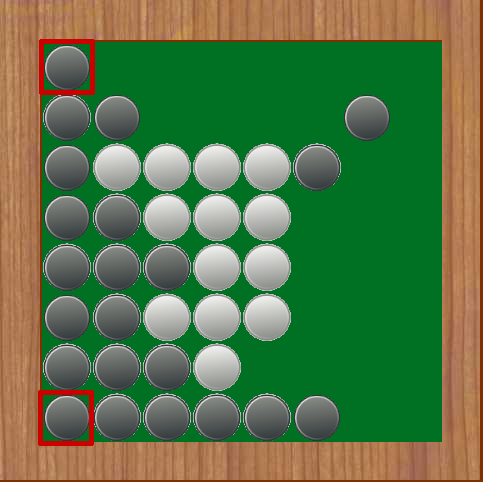
\includegraphics[width=0.8\textwidth]{img/screenshoot/raisonneur_choix_1}	
		}
		\only<3|handout:1>{
			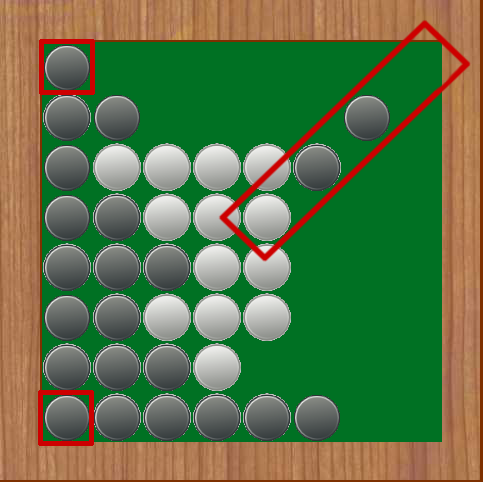
\includegraphics[width=0.8\textwidth]{img/screenshoot/raisonneur_choix_2}	
		}
	\end{minipage}
	\begin{minipage}{0.50\textwidth}
		\begin{itemize}
			\uncover<2->{
				\item $isCorner(x) \wedge isMine(x)$
			}
			\uncover<3->{
				\item $isMine(w) \wedge isOpp(x) \wedge isOpp(y) \wedge aligned(w,x,y) \wedge isEmpty(z) \wedge aligned (x,y,z)$
			}
		\end{itemize}
	\end{minipage}
\end{frame}

\begin{frame}{Raisonneur}{Moteur de choix}
	\begin{minipage}{0.45\textwidth}
		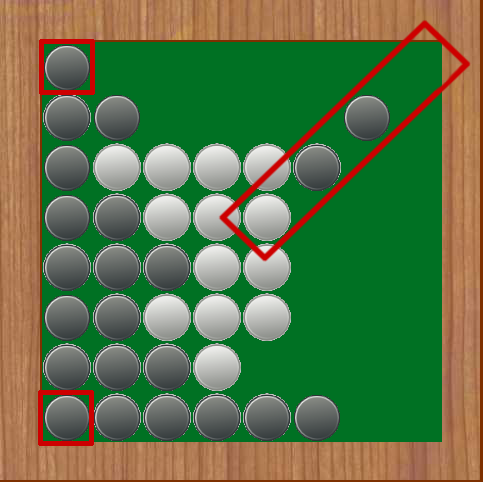
\includegraphics[width=0.8\textwidth]{img/screenshoot/raisonneur_choix_2}	
	\end{minipage}
	\begin{minipage}{0.50\textwidth}
		\begin{itemize}
			\item Moyenne de la probabilité de gain de chaque forme reconnue : $\overline{P(Gain|Forme)}$
		\end{itemize}
	\end{minipage}
\end{frame}

\begin{frame}{Raisonneur}{Valuation des formes}
	\begin{itemize}
			\item Valuation d'une forme :
			\[ P(Gain|Forme) = \frac{P(Forme|Gain) \times P(Gain)}{P(Forme)} \]\\[20pt]
			\item Fin de partie $\rightarrow$ mise à jour des formes rencontrées
		\end{itemize}
\end{frame}

\begin{frame}{Raisonneur}{Moteur d'introspection}
	Extraction de nouvelles formes
	\begin{center}
		\only<1|handout:0>{
			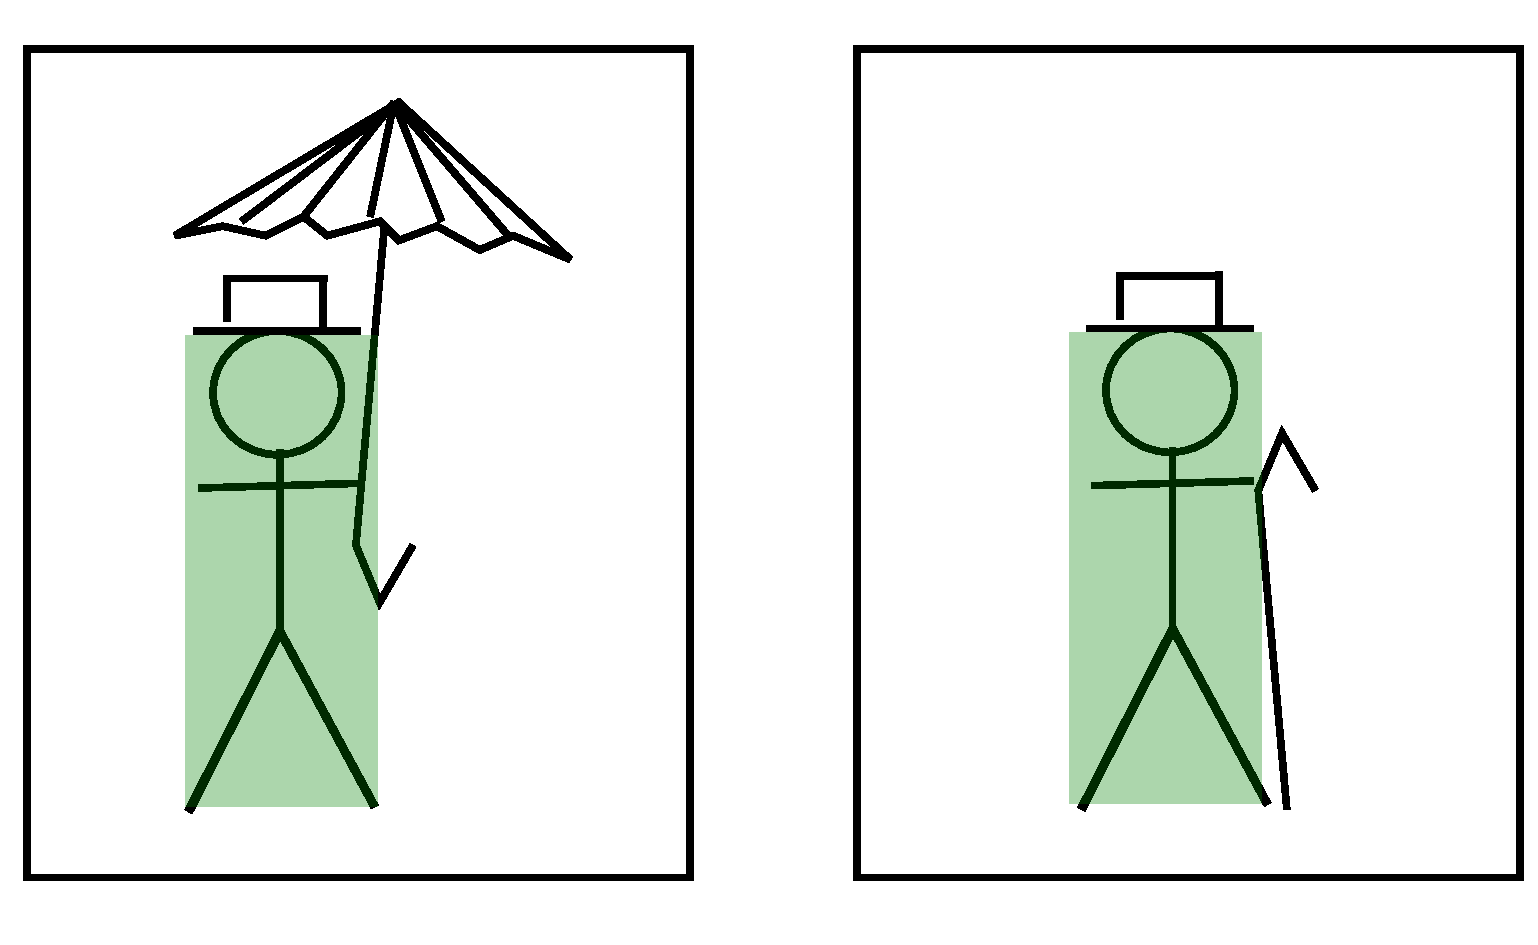
\includegraphics[width=0.8\textwidth]{img/raisonneur/reconnaissance_de_formes_2}	
		}
		\only<2|handout:0>{
			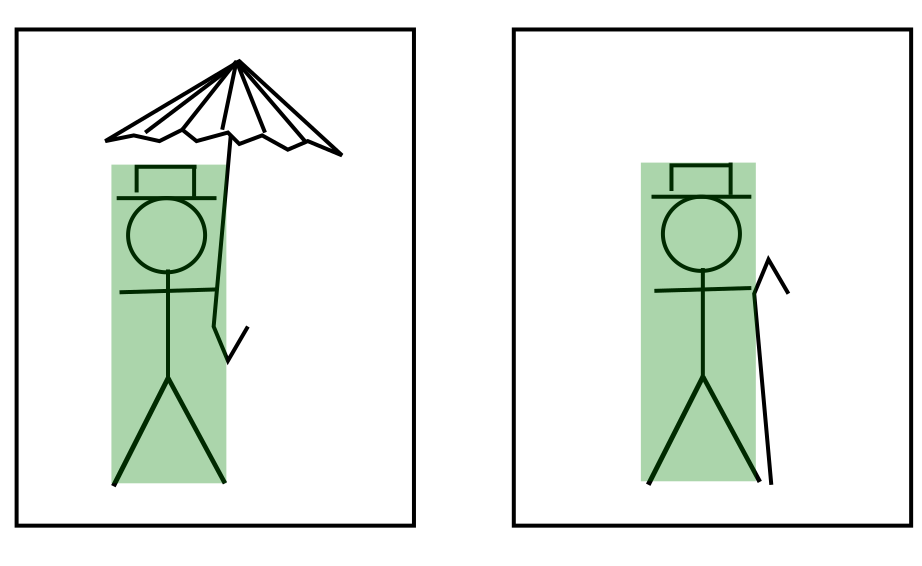
\includegraphics[width=0.8\textwidth]{img/raisonneur/reconnaissance_de_formes_1}	
		}
		\only<3|handout:0>{
			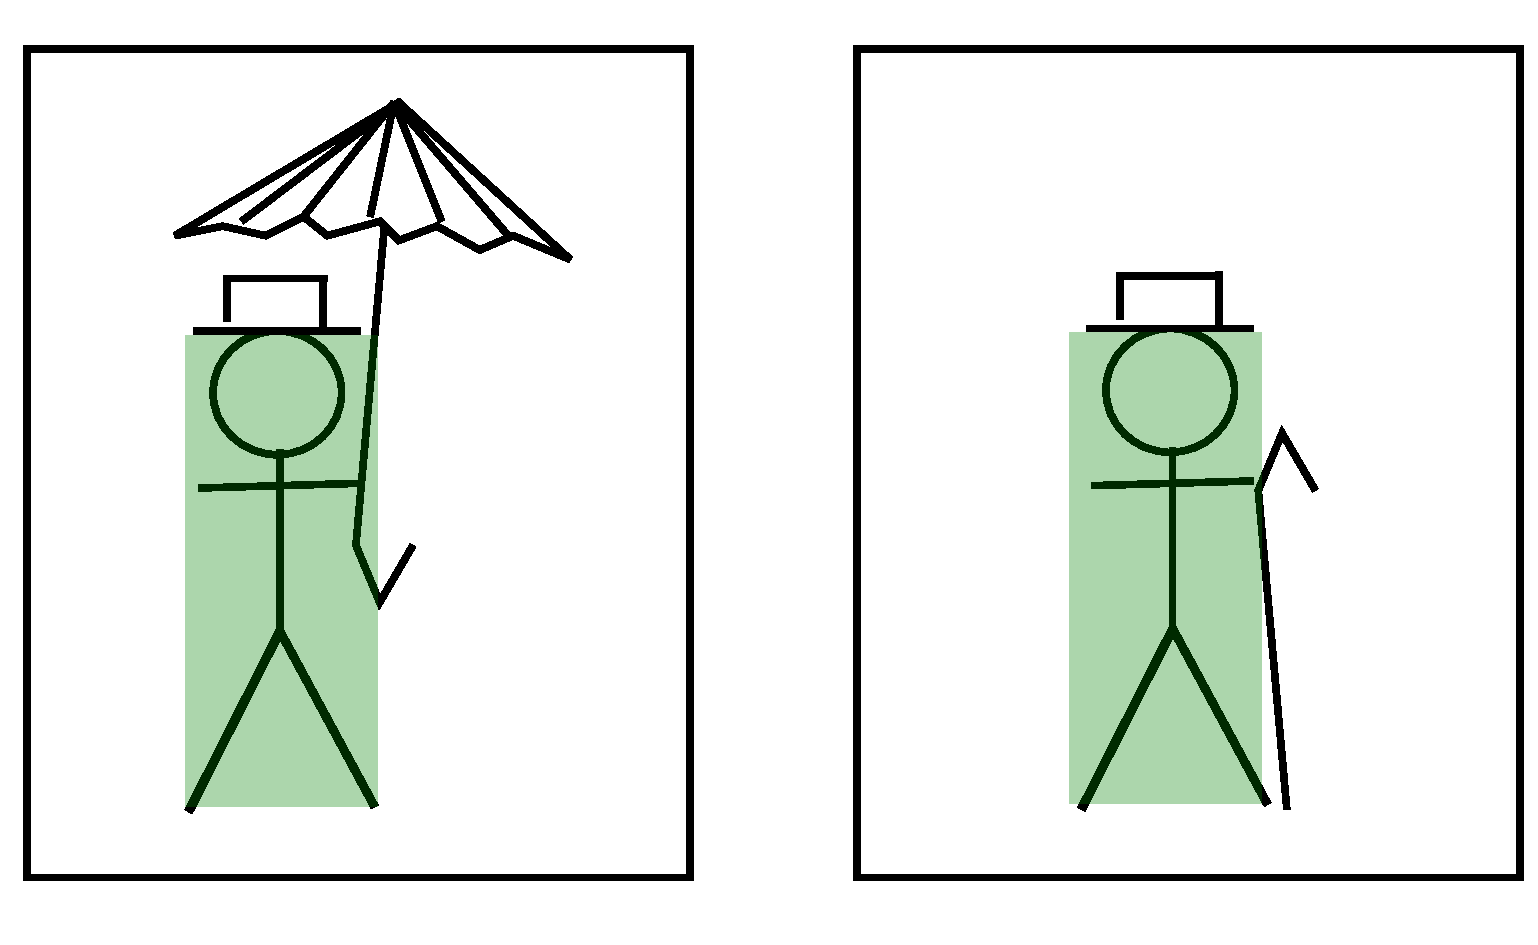
\includegraphics[width=0.8\textwidth]{img/raisonneur/reconnaissance_de_formes_2}	
		}
		\only<4|handout:1>{
			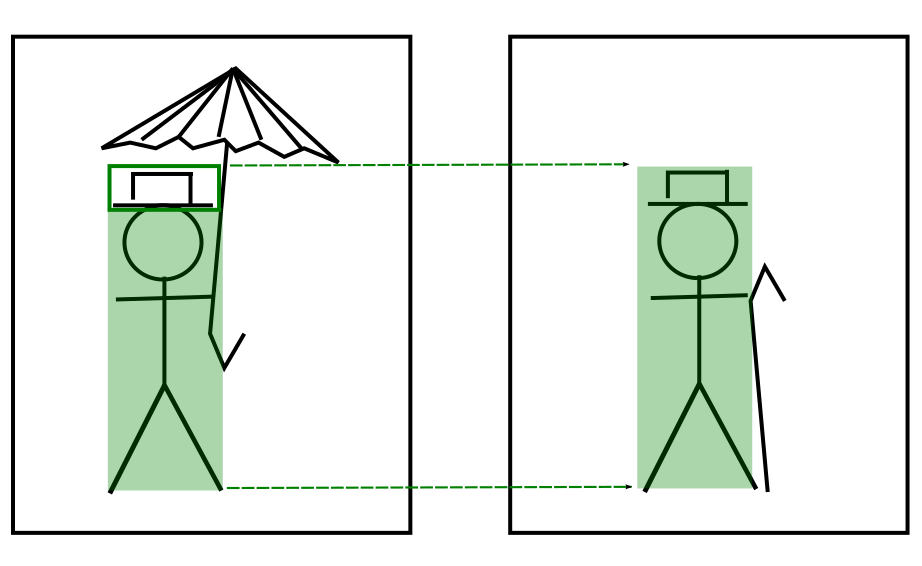
\includegraphics[width=0.8\textwidth]{img/raisonneur/reconnaissance_de_formes_injection}	
		}
	\end{center}
\end{frame}

\begin{frame}{Raisonneur}{Moteur d'introspection}
	\begin{minipage}{1\textwidth}
		\begin{minipage}{0.25\textwidth}
			\only<1|handout:0>{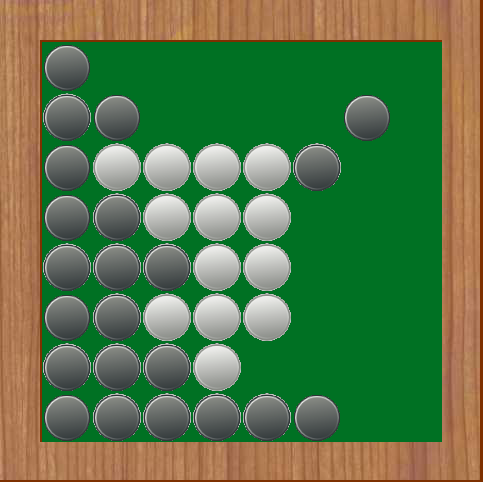
\includegraphics[width=\textwidth]{img/screenshoot/cbs0_reco0}	}
			\only<2|handout:0>{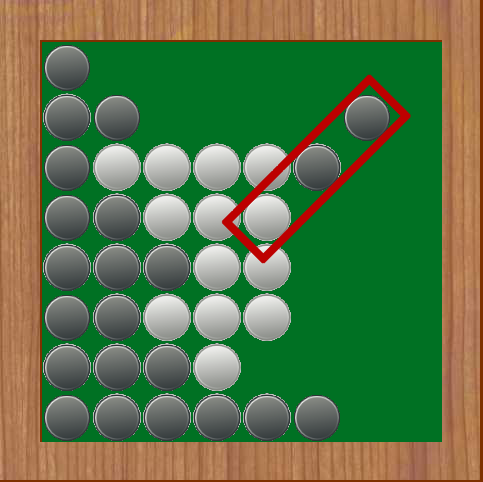
\includegraphics[width=\textwidth]{img/screenshoot/cbs0_reco1}	}
			\only<3-4|handout:1>{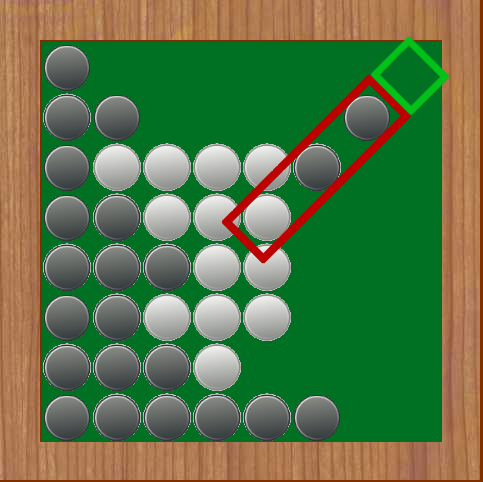
\includegraphics[width=\textwidth]{img/screenshoot/cbs0_reco2}	}
		\end{minipage}
		\begin{minipage}{0.75\textwidth}
			\only<2|handout:0>{$\ldots isMine(x0) \wedge isOpp(x1) \wedge isOpp(x2) \wedge aligned(x0,x1,x2)  \ldots $}
			\only<3-4|handout:1>{$\ldots isMine(x0) \wedge isOpp(x1) \wedge isOpp(x2) \wedge aligned(x0,x1,x2) \wedge isEmpty(x3) \wedge aligned (x1,x2,x3)			\wedge isCorner(x3) \ldots$}
		\end{minipage}
	\end{minipage}
	\\[10pt]
	\begin{minipage}{1\textwidth}
		\begin{minipage}{0.25\textwidth}
			\only<1|handout:0>{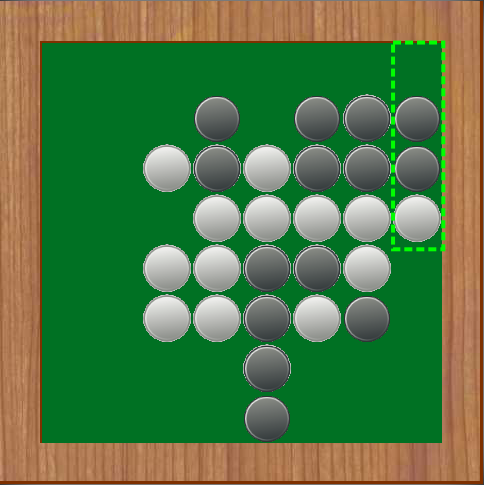
\includegraphics[width=\textwidth]{img/screenshoot/cbs1_reco0}	}
			\only<2-3|handout:0>{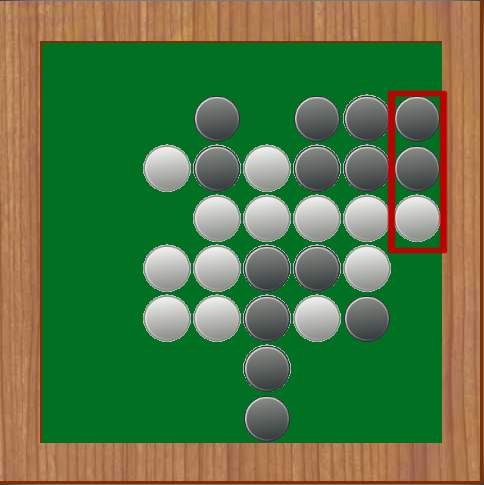
\includegraphics[width=\textwidth]{img/screenshoot/cbs1_reco1}	}
			\only<4|handout:1>{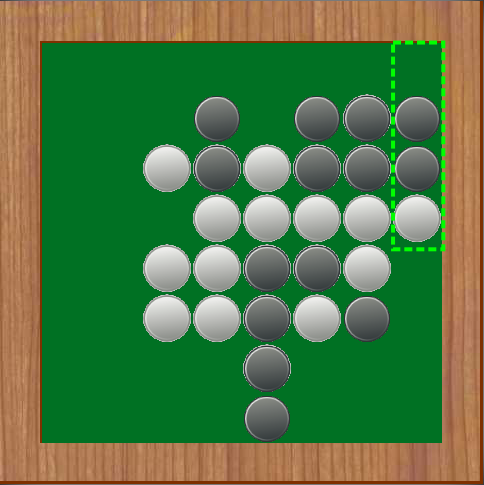
\includegraphics[width=\textwidth]{img/screenshoot/cbs1_reco2}	}		
		\end{minipage}
		\begin{minipage}{0.75\textwidth}
			\only<2-3|handout:0>{$\ldots isMine(y0) \wedge isOpp(y1) \wedge isOpp(y2) \wedge aligned(y0,y1,y2)  \ldots $}
			\only<4|handout:1>{$\ldots isMine(y0) \wedge isOpp(y1) \wedge isOpp(y2) \wedge aligned(y0,y1,y2) \wedge isEmpty(y3) \wedge aligned (y1,y2,y3) \wedge isCorner(y3) \ldots$}
		\end{minipage}
	\end{minipage}
\end{frame}
